\documentclass[12pt]{article}
\usepackage[margin=2.5cm]{geometry}
\usepackage{enumerate}
\usepackage{amsfonts}
\usepackage{amsmath}
\usepackage{fancyhdr}
\usepackage{amsmath}
\usepackage{amssymb}
\usepackage{amsthm}
\usepackage{mdframed}
\usepackage{graphicx}
\usepackage{subcaption}
\usepackage{adjustbox}
\usepackage{listings}
\usepackage{xcolor}
\usepackage{booktabs}
\usepackage[utf]{kotex}

\definecolor{codegreen}{rgb}{0,0.6,0}
\definecolor{codegray}{rgb}{0.5,0.5,0.5}
\definecolor{codepurple}{rgb}{0.58,0,0.82}
\definecolor{backcolour}{rgb}{0.95,0.95,0.92}

\lstdefinestyle{mystyle}{
    backgroundcolor=\color{backcolour},
    commentstyle=\color{codegreen},
    keywordstyle=\color{magenta},
    numberstyle=\tiny\color{codegray},
    stringstyle=\color{codepurple},
    basicstyle=\ttfamily\footnotesize,
    breakatwhitespace=false,
    breaklines=true,
    captionpos=b,
    keepspaces=true,
    numbers=left,
    numbersep=5pt,
    showspaces=false,
    showstringspaces=false,
    showtabs=false,
    tabsize=1
}

\lstset{style=mystyle}

\pagestyle{fancy}
\renewcommand{\headrulewidth}{0.4pt}
\lhead{Hyungmo Gu}
\rhead{CSC209 Week 9 Notes}

\begin{document}
\title{CSC209 Week 9 Notes}
\author{Hyungmo Gu}
\maketitle

\section*{Signals 1 of 2}

\bigskip

\begin{itemize}
    \item Introduction to Signals
    \begin{itemize}
        \item Signals
        \begin{itemize}
            \item are mechanisms that allow process or the os to interrupt
        currently running process and notify that an event has occured
        \end{itemize}

        \begin{center}
        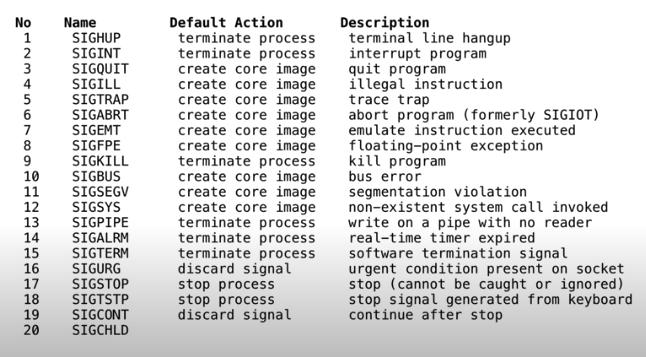
\includegraphics[width=\linewidth]{images/week_9_notes_1_1.png}
        \end{center}

        \item How it Works

        \begin{enumerate}[1.]
            \item Using hotkey
            \begin{itemize}
                \item i.e. \textit{CTRL + C} in terminal sends SIGINT
                \item i.e. \textit{CTRL + Z} in terminal sends SIGSTOP
            \end{itemize}

            \item Using kill command

            \begin{center}
            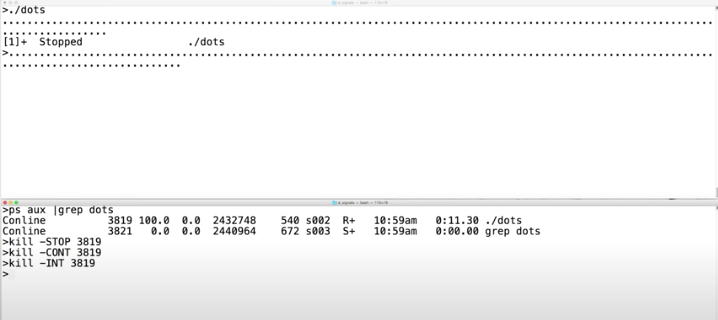
\includegraphics[width=\linewidth]{images/week_9_notes_1_2.png}
            \end{center}

    \begin{lstlisting}[language=bash]
    >>>./signals_example_1.out # <- This is done in separate terminal
    >>> ps aux | grep ./signals_example_1.out
    >>> kill -STOP <PID>
    >>> kill -CONT <PID>
    >>> kill -INT <PID>
    \end{lstlisting}

        \end{enumerate}
    \end{itemize}
\end{itemize}

\bigskip

\section*{Signals 2 of 2}

\bigskip

\begin{itemize}
    \item Signals Handling
    \begin{itemize}
        \item sigaction
        \begin{itemize}
            \item \textbf{Syntax:} int sigaction(int signum, const struct sigaction *act,
            NULL);
            \item Is a part of \textit{signal.h} library
            \item Is used to change the action taken by a process on receipt of
            a specific signal
            \item Works like try and catch in Python
            \item Don't worry about NULL :). Not knowing won't bite.
        \end{itemize}

        \bigskip

    \begin{lstlisting}[language=c]
    #include <stdio.h>
    #include <stdlib.h>
    #include <signal.h>

    void handler(int);

    int main () {
        struct sigaction newact;
        newact.sa_handler = handler; // <- like catch statement in python
        newact.sa_flags = 0;
        sigemptyset(&newact.sa_mask);
        return(0);
    }

    void handler(int code) {
        fprintf(stderr, "Signal %d caught\n", code);
    }
    \end{lstlisting}

        \begin{itemize}
            \item Use \textit{CTRL + Z} to terminate
            \item \textit{kill -KILL \textless PID \textgreater} and \textit{kill -QUIT \textless PID \textgreater}
            are two guarenteed ways to terminate a program.
        \end{itemize}

    \end{itemize}
\end{itemize}

\bigskip

\section*{Bit Manipulation 1 of 4}

\bigskip

\begin{itemize}
    \item Introducing Bitwise Operations
    \begin{itemize}
        \item When to use Bitwise Operations?
        \begin{itemize}
            \item Lowlevel programming on embedded systems
        \end{itemize}
        \item Bitwise Operators in C
        \begin{itemize}
            \item \textbf{\&:} AND

            \bigskip

            \begin{center}
                \begin{tabular}{|c|c|c|}
                    \hline
                    a & b & a \& b\\
                    \hline
                    0 & 0  & 0 \\
                    0 & 1  & 1 \\
                    1 & 0  & 0 \\
                    1 & 1  & 1 \\
                    \hline
                \end{tabular}
            \end{center}

            \bigskip

            \textbf{Example:}

            \bigskip

    \begin{lstlisting}[language=c]
    0   1   1   1   //<- this is 7
    0   1   0   0   //<- this is 4
    --------------
    0   1   0   0   //<- this is 4

    so, 7 & 4 = 4
    \end{lstlisting}

            \item \textbf{$\mid$:} OR

            \bigskip

            \begin{center}
                \begin{tabular}{|c|c|c|}
                    \hline
                    a & b & a $\mid$ b\\
                    \hline
                    0 & 0  & 0 \\
                    0 & 1  & 1 \\
                    1 & 0  & 1 \\
                    1 & 1  & 1 \\
                    \hline
                \end{tabular}
            \end{center}

            \bigskip

            \textbf{Example:}

            \bigskip

    \begin{lstlisting}[language=c]
    0   1   1   1   //<- this is 7
    0   1   0   0   //<- this is 4
    --------------
    0   1   1   1   //<- this is 7

    so, 7 | 4 = 4
    \end{lstlisting}


            \item \textbf{~:} NOT

            \bigskip

            \begin{center}
                \begin{tabular}{|c|c|c|}
                    \hline
                    a & $\sim$ a\\
                    \hline
                    0 & 1\\
                    1 & 0\\
                    \hline
                \end{tabular}
            \end{center}

            \bigskip

            \textbf{Example:}

            \bigskip

    \begin{lstlisting}[language=c]
    0   1   1   1   //<- this is 7
    --------------
    1   0   0   0   //<- this is 8

    so, ~ 7 = 8
    \end{lstlisting}

            \item \textbf{\^:} XOR

            \bigskip

            \begin{center}
                \begin{tabular}{|c|c|c|}
                    \hline
                    a & b & a \^{} b\\
                    \hline
                    0 & 0  & 0 \\
                    0 & 1  & 1 \\
                    1 & 0  & 1 \\
                    1 & 1  & 0 \\
                    \hline
                \end{tabular}
            \end{center}

            \bigskip

            \textbf{Example:}

            \bigskip

    \begin{lstlisting}[language=c]
    0   1   1   1   //<- this is 7
    0   1   0   0   //<- this is 4
    --------------
    0   0   1   1   //<- this is 3

    so, 7 ^ 4 = 3
    \end{lstlisting}
        \end{itemize}
    \end{itemize}
\end{itemize}

\bigskip

\section*{Bit Manipulation 2 of 4}

\bigskip

\begin{itemize}
    \item Hexadecimal Numbers
    \begin{itemize}
        \item Starts with `0x' at front
        \begin{itemize}
            \item `0x` is for uncapitalized letters, i.e. `0XFFFF`
            \item `0X' is for capitalized letters, i.e. 0xffff
        \end{itemize}
        \item Uses 10 symbols `$0,1,2,3,4,5,6,7,8,9$' and 6 extras `$A = 10, B = 11, C = 12, D = 13, E = 14, F = 15$'.
        \begin{itemize}
            \item i.e. $0xFFFF =  15 \cdot 16^0 + 15 \cdot 16^1 + 15 \cdot 16^2 + 15 \cdot 16^3 + 15 \cdot 16^4 = 65535$
        \end{itemize}
    \end{itemize}
    \item The Shift Operators
    \begin{itemize}
        \item \textbf{\textless\textless $n$:} LEFT SHIFT

        \begin{itemize}
            \item Shifts all bits to left by $n$
        \end{itemize}

        \bigskip

        \textbf{Example:}

        \bigskip

\begin{lstlisting}[language=c]
i = 7
j = i << 1

0   1   1   1   //<- this is 7
--------------
1   1   1   0   //<- this is 14

so, 7 << 1 = 14
\end{lstlisting}

        \item \textbf{\textgreater\textgreater $n$:} RIGHT SHIFT
        \begin{itemize}
            \item Shifts all bits to right by $n$
        \end{itemize}

        \bigskip

        \textbf{Example:}

        \bigskip

\begin{lstlisting}[language=c]
i = 7
j = i >> 1

0   1   1   1   //<- this is 7
--------------
0   0   1   1   //<- this is 3

so, 7 >> 1 = 3
\end{lstlisting}
    \end{itemize}
\end{itemize}

\bigskip

\section*{Bit Manipulation 3 of 4}

\bigskip

\begin{itemize}
    \item Bit Flags
    \begin{itemize}
        \item Bit flags are boolean variables represented using 0 and 1
        \begin{itemize}
            \item bool variables consume 1 byte (8 bits)
            \item 0 or 1 consume 1 bit
        \end{itemize}
        \item Use of Bit Flags
        \begin{itemize}
            \item Embedded Software Programming
            \item Graphics card
        \end{itemize}
        \item Example
        \begin{enumerate}[1.]
            \item chmod and unix file system

            \begin{center}
            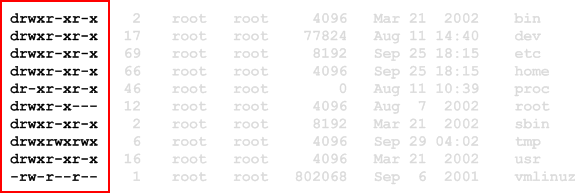
\includegraphics[width=\linewidth]{images/week_9_notes_3_1.png}
            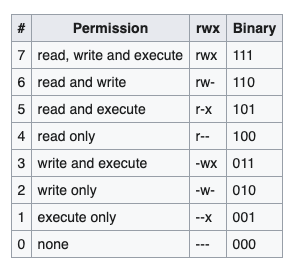
\includegraphics[width=0.4\linewidth]{images/week_9_notes_3_2.png}
            \end{center}

            \bigskip

            \begin{enumerate}[1.]
                \item Setting read-only permission to a file to owner
    \begin{lstlisting}[language=c]
    r--------
    100000000 // <- Binary
    [4]  [0]  [0]   // <- Octal

    chmod 400 <file>
    \end{lstlisting}
            \item Setting read and write only permissions to a file
    \begin{lstlisting}[language=c]
    rw-rw-rw-
    110110110 // <- Binary
    [4+2=6] [4+2=6] [4+2=6]  // <- Octal

    chmod 666 <file>
    \end{lstlisting}

            \item Setting all permissions to a file
    \begin{lstlisting}[language=c]
    rwxrwxrwx
    110110110 // <- Binary
    [4+2+1=7] [4+2+1=7] [4+2+1=7]  // <- Octal

    chmod 777 <file>
    \end{lstlisting}
            \end{enumerate}
        \end{enumerate}

    \end{itemize}

    \item Octal Bit Flags in C
    \begin{itemize}
        \item Are written with preecding 0

        \begin{center}
        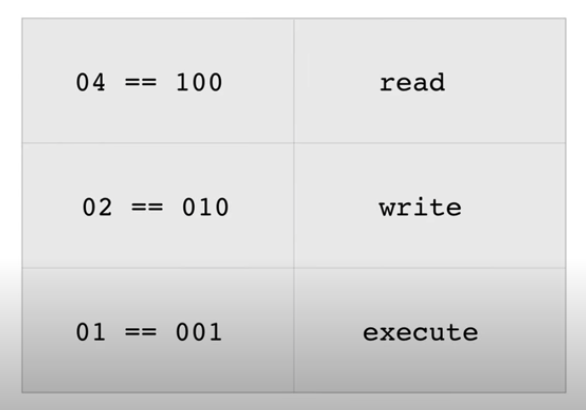
\includegraphics[width=0.6\linewidth]{images/week_9_notes_3_3.png}
        \end{center}

\begin{lstlisting}[language=c]
#include <stdio.h>
#include <unistd.h>
#include <stdio.h>

#define S_IRUSR 0000400 //R for owner
#define S_IRGRP 0000400 //R for group
#define S_IROTH 0000400 //R for others

int main () {
    mode_t mode = S_IRUSR | S_IRGRP | S_IROTH; // Example 1
    mode_t mode = 0400 | 040 | 004; // Example 2 (<- Notice bitwise or is used)
    mode_t mode = 0444; // Example 3
    return(0);
}
\end{lstlisting}

    \end{itemize}
\end{itemize}



\bigskip

\section*{Bit Manipulation 4 of 4}

\bigskip

\begin{itemize}
    \item Bit array
    \begin{itemize}
        \item Reduces usage of space
        \begin{itemize}
        \item Traditional array uses 32 bits per slot
        \item Bit array uses 1 bits per slot
        \end{itemize}
    \end{itemize}
    \item Bit Masking
    \begin{itemize}
        \item is a technique to add/remove specific element in bit array
        \item \textbf{Adding element} $\to$ Bitwise OR

        \begin{center}
        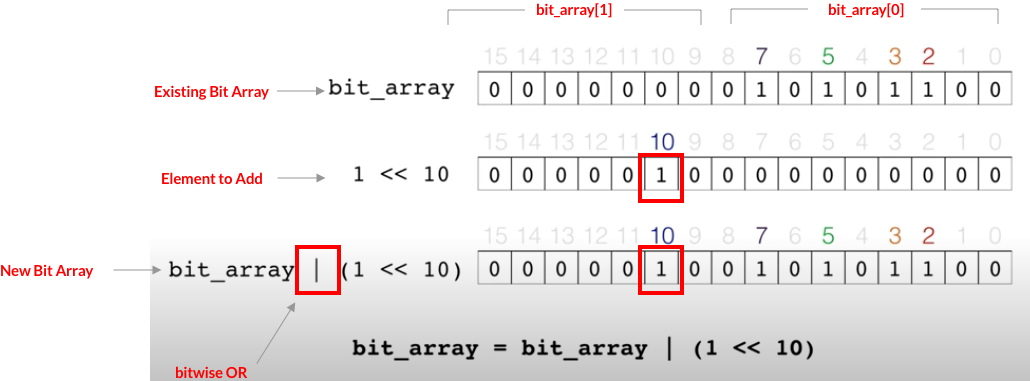
\includegraphics[width=\linewidth]{images/week_9_notes_4_1.png}
        \end{center}
        \item \textbf{Removing element} $\to$ Bitwise AND

        \begin{center}
        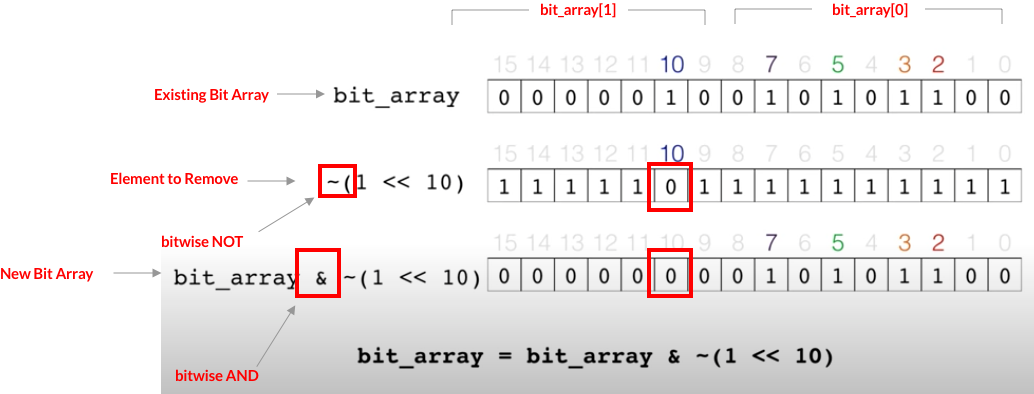
\includegraphics[width=\linewidth]{images/week_9_notes_4_2.png}
        \end{center}

        \item General Rule
        \begin{enumerate}[1.]
            \item Create Bit array

    \begin{lstlisting}[language=c]
    #define N 4

    unsigned bit_array[N];
    \end{lstlisting}
            \item Determine target position $k$ of element in unsigned array
    \begin{lstlisting}[language=c]
    int i = k/N;
    \end{lstlisting}
            \item Determine which bit in element to modify

    \begin{lstlisting}[language=c]
    int pos = k%N;
    \end{lstlisting}

            \item Complete by performing Bitwise OR/AND

    \begin{lstlisting}[language=c]
    flag = 1 << pos; // <- ~(1 << pos) if performing Bitwise AND
    bit_array[i] = bit_array[i] | flag;
    \end{lstlisting}

        \item More details: http://www.mathcs.emory.edu/~cheung/Courses/255/Syllabus/1-C-intro/bit-array.html
        \end{enumerate}
    \end{itemize}

    \begin{lstlisting}[language=c,caption={bit\_manipulation\_example\_4.c}]
    #include <stdio.h>
    #include <unistd.h>
    #include <stdlib.h>
    #include <string.h>
    #include <sys/types.h>
    #include <stdio.h>

    #define INTSIZE 32
    #define N 4

    typedef struct bits {
        unsigned int field[N];
    } Bitarray;

    int setzero(Bitarray *b) {
        return (memset(b, 0, sizeof(Bitarray)) == NULL);
    }

    void set(unsigned int value, Bitarray *b) {
        int index = value / INTSIZE;
        b->field[index] |= 1 << (value % INTSIZE);
    }


    void unset(unsigned int value, Bitarray *b) {
        int index = value / INTSIZE;
        b->field[index] &= ~(1 << (value % INTSIZE));
    }

    int ifset(unsigned int value, Bitarray *b) {
        int index = value / INTSIZE;
        return (1 << (value % INTSIZE) & b->field[index]);
    }


    int main () {
        Bitarray a1;
        setzero(&a1);

        // Add 1, 16, 32, 65 to the set
        set(1, &a1);
        set(16, &a1);
        set(32, &a1);
        set(65, &a1);

        // expecting: [0x00010002, 0x00000001, 0x000000010, 0]
        printf("%x %x %x %x\n",
            a1.field[0], a1.field[1], a1.field[2], a1.field[3]);
    }

    \end{lstlisting}

\end{itemize}

\end{document}